\documentclass[11pt]{article}
\usepackage[final]{acl}
\usepackage{times}
\usepackage{latexsym}
\usepackage[T1]{fontenc}
\usepackage[utf8]{inputenc}
\usepackage{microtype}
\usepackage{inconsolata}
\usepackage{graphicx}
\usepackage{booktabs}
\usepackage{amsmath}

\newcommand{\AgreementSentence}{Two team members labelled 100 random pairs blind to the automatic label: Cohen's $\kappa$ = 0.61 between them and 0.54 and 0.58 with the automatic labels (raw agreement 0.77).}
\newcommand{\TestNSandboxBinary}{219}
\newcommand{\TestNSandboxThree}{306}
\newcommand{\TestNScienceWorldBinary}{235}
\newcommand{\TestNScienceWorldThree}{238}
\newcommand{\RQFiveN}{776}
\newcommand{\QwenSevenLayer}{20}
\newcommand{\QwenSevenLayers}{28}
\newcommand{\QwenSevenProbeSandbox}{0.984}
\newcommand{\QwenSevenProbeSandboxMin}{0.979}
\newcommand{\QwenSevenProbeSW}{0.945}
\newcommand{\QwenSevenProbeThree}{0.906}
\newcommand{\QwenSevenTransferSbSw}{0.475}
\newcommand{\QwenSevenTransferSwSb}{0.500}
\newcommand{\QwenSevenStatedSandbox}{0.38}
\newcommand{\QwenSevenStatedSW}{0.38}
\newcommand{\QwenSevenKappaProbe}{0.11}
\newcommand{\QwenSevenSaysIrrevSandbox}{84}
\newcommand{\QwenSevenSaysRevSandbox}{16}
\newcommand{\QwenSevenSaysIrrevSW}{100}
\newcommand{\QwenSevenSaysRevSW}{0}
\newcommand{\QwenSevenGapNeutral}{0.20}
\newcommand{\QwenSevenGapNeutralCI}{[0.10, 0.30]}
\newcommand{\QwenSevenSensNeutral}{0.00}
\newcommand{\QwenSevenKNeutral}{0.20}
\newcommand{\QwenSevenANeutral}{0.00}
\newcommand{\QwenSevenCautionNeutral}{0.22}
\newcommand{\QwenSevenParseNeutral}{20}
\newcommand{\QwenSevenGapCareful}{0.20}
\newcommand{\QwenSevenGapCarefulCI}{[0.10, 0.30]}
\newcommand{\QwenSevenSensCareful}{0.00}
\newcommand{\QwenSevenKCareful}{0.20}
\newcommand{\QwenSevenACareful}{0.00}
\newcommand{\QwenSevenCautionCareful}{0.22}
\newcommand{\QwenSevenParseCareful}{6}
\newcommand{\QwenSevenCarefulP}{=1}
\newcommand{\QwenSevenSMax}{6}
\newcommand{\QwenSevenSteerProbeNeg}{0.30}
\newcommand{\QwenSevenSteerProbeNegSuccess}{0.93}
\newcommand{\QwenSevenSteerProbeNegParse}{104}
\newcommand{\QwenSevenSteerProbePos}{0.00}
\newcommand{\QwenSevenSteerProbePosSuccess}{0.93}
\newcommand{\QwenSevenSteerProbePosParse}{2}
\newcommand{\QwenSevenSteerRandomNeg}{0.23}
\newcommand{\QwenSevenSteerRandomNegSuccess}{0.92}
\newcommand{\QwenSevenSteerRandomNegParse}{20}
\newcommand{\QwenSevenSteerRandomPos}{0.17}
\newcommand{\QwenSevenSteerRandomPosSuccess}{0.92}
\newcommand{\QwenSevenSteerRandomPosParse}{31}
\newcommand{\QwenSevenSteerZero}{0.22}
\newcommand{\QwenSevenRQFiveAUROC}{0.56}
\newcommand{\QwenSevenRQFiveGold}{0.54}
\newcommand{\QwenSevenToolEmuProbe}{0.80}
\newcommand{\QwenSevenToolEmuAUROC}{0.89}
\newcommand{\QwenSevenToolEmuStated}{0.58}
\newcommand{\QwenSevenToolEmuGap}{0.06}
\newcommand{\QwenSevenToolEmuGapCI}{[$-$0.02, 0.15]}
\newcommand{\QwenSevenToolEmuSens}{0.00}
\newcommand{\QwenSevenToolEmuIrrAct}{0.98}
\newcommand{\LlamaEightLayer}{10}
\newcommand{\LlamaEightLayers}{32}
\newcommand{\LlamaEightProbeSandbox}{0.981}
\newcommand{\LlamaEightProbeSandboxMin}{0.975}
\newcommand{\LlamaEightProbeSW}{0.942}
\newcommand{\LlamaEightProbeThree}{0.903}
\newcommand{\LlamaEightTransferSbSw}{0.541}
\newcommand{\LlamaEightTransferSwSb}{0.496}
\newcommand{\LlamaEightStatedSandbox}{0.45}
\newcommand{\LlamaEightStatedSW}{0.67}
\newcommand{\LlamaEightKappaProbe}{0.10}
\newcommand{\LlamaEightSaysIrrevSandbox}{13}
\newcommand{\LlamaEightSaysRevSandbox}{60}
\newcommand{\LlamaEightSaysIrrevSW}{23}
\newcommand{\LlamaEightSaysRevSW}{76}
\newcommand{\LlamaEightGapNeutral}{0.10}
\newcommand{\LlamaEightGapNeutralCI}{[$-$0.07, 0.25]}
\newcommand{\LlamaEightSensNeutral}{0.02}
\newcommand{\LlamaEightKNeutral}{0.27}
\newcommand{\LlamaEightANeutral}{0.17}
\newcommand{\LlamaEightCautionNeutral}{0.32}
\newcommand{\LlamaEightParseNeutral}{2}
\newcommand{\LlamaEightGapCareful}{0.03}
\newcommand{\LlamaEightGapCarefulCI}{[$-$0.12, 0.18]}
\newcommand{\LlamaEightSensCareful}{0.08}
\newcommand{\LlamaEightKCareful}{0.27}
\newcommand{\LlamaEightACareful}{0.23}
\newcommand{\LlamaEightCautionCareful}{0.70}
\newcommand{\LlamaEightParseCareful}{5}
\newcommand{\LlamaEightCarefulP}{<0.001}
\newcommand{\LlamaEightSMax}{6}
\newcommand{\LlamaEightSteerProbeNeg}{0.55}
\newcommand{\LlamaEightSteerProbeNegSuccess}{0.68}
\newcommand{\LlamaEightSteerProbeNegParse}{0}
\newcommand{\LlamaEightSteerProbePos}{0.05}
\newcommand{\LlamaEightSteerProbePosSuccess}{0.93}
\newcommand{\LlamaEightSteerProbePosParse}{0}
\newcommand{\LlamaEightSteerRandomNeg}{0.38}
\newcommand{\LlamaEightSteerRandomNegSuccess}{0.88}
\newcommand{\LlamaEightSteerRandomNegParse}{0}
\newcommand{\LlamaEightSteerRandomPos}{0.30}
\newcommand{\LlamaEightSteerRandomPosSuccess}{0.83}
\newcommand{\LlamaEightSteerRandomPosParse}{8}
\newcommand{\LlamaEightSteerZero}{0.32}
\newcommand{\LlamaEightRQFiveAUROC}{0.53}
\newcommand{\LlamaEightRQFiveGold}{0.50}
\newcommand{\LlamaEightToolEmuProbe}{0.76}
\newcommand{\LlamaEightToolEmuAUROC}{0.84}
\newcommand{\LlamaEightToolEmuStated}{0.45}
\newcommand{\LlamaEightToolEmuGap}{0.09}
\newcommand{\LlamaEightToolEmuGapCI}{[$-$0.04, 0.22]}
\newcommand{\LlamaEightToolEmuSens}{0.04}
\newcommand{\LlamaEightToolEmuIrrAct}{1.00}
\newcommand{\QwenFourteenLayer}{29}
\newcommand{\QwenFourteenLayers}{48}
\newcommand{\QwenFourteenProbeSandbox}{0.990}
\newcommand{\QwenFourteenProbeSandboxMin}{0.987}
\newcommand{\QwenFourteenProbeSW}{0.942}
\newcommand{\QwenFourteenProbeThree}{0.914}
\newcommand{\QwenFourteenTransferSbSw}{0.540}
\newcommand{\QwenFourteenTransferSwSb}{0.537}
\newcommand{\QwenFourteenStatedSandbox}{0.66}
\newcommand{\QwenFourteenStatedSW}{0.66}
\newcommand{\QwenFourteenKappaProbe}{0.46}
\newcommand{\QwenFourteenSaysIrrevSandbox}{26}
\newcommand{\QwenFourteenSaysRevSandbox}{41}
\newcommand{\QwenFourteenSaysIrrevSW}{19}
\newcommand{\QwenFourteenSaysRevSW}{69}
\newcommand{\QwenFourteenGapNeutral}{0.65}
\newcommand{\QwenFourteenGapNeutralCI}{[0.53, 0.78]}
\newcommand{\QwenFourteenSensNeutral}{$-$0.02}
\newcommand{\QwenFourteenKNeutral}{0.67}
\newcommand{\QwenFourteenANeutral}{0.02}
\newcommand{\QwenFourteenCautionNeutral}{0.02}
\newcommand{\QwenFourteenParseNeutral}{1}
\newcommand{\QwenFourteenGapCareful}{0.63}
\newcommand{\QwenFourteenGapCarefulCI}{[0.52, 0.75]}
\newcommand{\QwenFourteenSensCareful}{0.00}
\newcommand{\QwenFourteenKCareful}{0.67}
\newcommand{\QwenFourteenACareful}{0.03}
\newcommand{\QwenFourteenCautionCareful}{0.05}
\newcommand{\QwenFourteenParseCareful}{1}
\newcommand{\QwenFourteenCarefulP}{=0.5}
\newcommand{\QwenFourteenSMax}{6}
\newcommand{\QwenFourteenSteerProbeNeg}{0.52}
\newcommand{\QwenFourteenSteerProbeNegSuccess}{0.48}
\newcommand{\QwenFourteenSteerProbeNegParse}{12}
\newcommand{\QwenFourteenSteerProbePos}{0.00}
\newcommand{\QwenFourteenSteerProbePosSuccess}{0.93}
\newcommand{\QwenFourteenSteerProbePosParse}{9}
\newcommand{\QwenFourteenSteerRandomNeg}{0.52}
\newcommand{\QwenFourteenSteerRandomNegSuccess}{0.97}
\newcommand{\QwenFourteenSteerRandomNegParse}{0}
\newcommand{\QwenFourteenSteerRandomPos}{0.10}
\newcommand{\QwenFourteenSteerRandomPosSuccess}{0.97}
\newcommand{\QwenFourteenSteerRandomPosParse}{10}
\newcommand{\QwenFourteenSteerZero}{0.02}
\newcommand{\QwenFourteenRQFiveAUROC}{0.59}
\newcommand{\QwenFourteenRQFiveGold}{0.60}
\newcommand{\QwenFourteenToolEmuProbe}{0.81}
\newcommand{\QwenFourteenToolEmuAUROC}{0.91}
\newcommand{\QwenFourteenToolEmuStated}{0.58}
\newcommand{\QwenFourteenToolEmuGap}{0.74}
\newcommand{\QwenFourteenToolEmuGapCI}{[0.61, 0.85]}
\newcommand{\QwenFourteenToolEmuSens}{0.00}
\newcommand{\QwenFourteenToolEmuIrrAct}{1.00}

% Author names and roll numbers.
\newcommand{\AuthorBlock}{%
  Anshika Mishra \\ SE23UCSE027 \And
  Banoth Rohith Rathod \\ SE23UCSE034 \AND
  Gonuguntla Rusheel \\ SE23UCSE067 \And
  Goyal Aditya \\ SE23UARI003}


\title{Knowing Without Acting: Do LLM Agents Represent\\Which Actions Cannot Be Undone?}

\author{\AuthorBlock}

\begin{document}
\maketitle

\begin{abstract}
Agents built on large language models delete files, send messages and move money, and nothing guarantees that they handle irreversible steps differently from reversible ones. We study three open-weight models (Qwen2.5-7B, Llama-3.1-8B and Qwen2.5-14B) and measure three things: whether a linear probe can decode the reversibility of a (state, action) pair from the hidden states, whether the model gives the right answer when asked, and whether it acts more carefully before irreversible actions. Our dataset has 2,648 labelled pairs from a tool sandbox and ScienceWorld. More than half are minimal pairs, in which the same action is reversible in one state and irreversible in another. From the middle layers on, the probe decodes reversibility in all three models (sandbox balanced accuracy \QwenSevenProbeSandbox{}--\QwenFourteenProbeSandbox{}; \LlamaEightProbeSandboxMin{}--\QwenFourteenProbeSandboxMin{} on minimal pairs, where a bag-of-words baseline is at chance). When asked, the two smaller models mostly give one default answer (three-class accuracy \QwenSevenStatedSandbox{} and \LlamaEightStatedSandbox{}), while Qwen2.5-14B is usually right (\QwenFourteenStatedSandbox{}). As agents on 60 paired tasks, none of the models is more careful in the irreversible version (reversibility sensitivity between $-0.02$ and $0.02$). The irreversibility blindness gap, stated knowledge minus careful behaviour, therefore grows with scale and reaches \QwenFourteenGapNeutral{} \QwenFourteenGapNeutralCI{} for the 14B model. In the two smaller models, steering along the probe direction changes caution, but it lowers it, and equally in both task versions. In the 14B model it does no more than a random direction. The probe does not transfer between environments, and next-state uncertainty is at most weakly related to reversibility.
\end{abstract}

\section{Introduction}

LLM agents now run commands, edit files, send messages and call payment tools. Some of these actions can be undone (moving a file to a recycle bin), some only partly (editing a file whose old text survives only in a history), and some not at all (sending an email, paying an invoice). A careful person slows down before the last kind. We ask whether LLM agents do too. If they do not, there are two explanations: they do not know which actions are irreversible, or they know and the knowledge does not affect what they choose. We call the second case \emph{irreversibility blindness}. A model with it can say that deleting a file is permanent and then delete it without checking anything.

We split the question into five measurements. RQ1: can a linear probe decode reversibility from the hidden state of the candidate action, and at which layers? RQ2: when asked in plain language, does the model give the right label, and does that answer agree with the probe? RQ3: as an agent, is the model more careful before irreversible actions? RQ4: does adding the probe's ``irreversible'' direction to the residual stream make the agent more careful? RQ5: is the model's uncertainty about the next state related to reversibility?

We contribute (i) a dataset of 2,648 (state, action) pairs, from a tool sandbox with exact reversibility and from ScienceWorld labelled by reset-and-replay search, 54.5\% of them minimal pairs; (ii) probes on three open-weight models with the usual controls, including a lexical baseline on minimal pairs, shuffled labels and a Hewitt--Liang control task; (iii) 60 paired agent tasks plus 54 ToolEmu cases rebuilt in the sandbox, which give a blindness gap with confidence intervals; and (iv) a causal steering test and an uncertainty test. In all three models reversibility is linearly decodable and has almost no effect on what the agent does. The gap between what the model says and what it does is largest for the 14B model.

\section{Related Work}

\paragraph{Reversibility in reinforcement learning.} \citet{grinsztajn2021turning} learn a self-supervised estimate of how likely a transition is to be reversed and use it to avoid irreversible actions; \citet{krakovna2018penalizing} and \citet{turner2020conservative} penalise side effects through reachability and attainable utility. These methods build reversibility into the agent. We ask whether a pretrained language model already represents it.

\paragraph{Risky actions of LLM agents.} ToolEmu \citep{ruan2024toolemu} emulates tools with an LLM to find risky agent behaviour, and SafeAgentBench \citep{yin2024safeagentbench} tests hazardous plans of embodied agents. \citet{tang2025risk} show that agents often fail to act on risk knowledge they can state. This is the closest result to ours, though it covers risk in general and does not look inside the model. AgentAbstain \citep{liu2026agentabstain} finds that agents often recognise only after an irreversible step that they should have abstained, and \citet{zhai2026revisable} classify agent actions by reversibility for streaming execution; neither probes internal representations. \citet{schmied2026greedy} describe a similar gap between knowing and doing in decision making.

\paragraph{Probes, controls and steering.} Linear probes read information from intermediate layers \citep{alain2016probes}. \citet{hewitt-liang-2019-designing} show that a probe can succeed by memorising, and introduce control tasks and selectivity to check for it. World-state representations in Othello-GPT turned out to be nonlinear \citep{li2023emergent}, so a linear probe can miss information that is present. Contrastive activation addition \citep{rimsky-etal-2024-steering} steers behaviour by adding a mean-difference direction; we use it for RQ4. For RQ5 we use the state-prediction data of \citet{wang-etal-2024-language}.

\section{Method}

\subsection{Testbeds and labels}

\paragraph{Tool sandbox.} A Python class holds files (with sizes, contents and revisions), a recycle bin, an external archive, backups, an email outbox and a wallet, and can save and restore its full state. Each of its 24 tools has a reversibility fixed by design. An action is \emph{reversible} if the exact previous state can be restored within 3 actions, \emph{partially reversible} if it can only be restored approximately or at a cost (a backup older than the current text, a refund minus a fee, an email recall that leaves a notice), and \emph{irreversible} otherwise. A breadth-first restore search checks the design labels in our tests. Minimal pairs put the same tool call in states that differ only in the setting that decides its reversibility: \texttt{delete\_file} with the recycle bin on or off, \texttt{edit\_file} with or without a backup or version history, \texttt{send\_email} with or without a 60-second undo window, and \texttt{transfer\_money} when the transfer is cancellable, refundable or final.

\paragraph{ScienceWorld.} ScienceWorld \citep{wang-etal-2022-scienceworld} has no save and restore, so we rebuild a state by resetting the task variation and replaying the action history. States are sampled from gold-path prefixes of all 30 tasks. For a state and an action, we compare the world after the action with a null baseline (the same number of no-op ticks) and search for restoring sequences of length up to $h=3$ (we also report $h=1,2$). Thermal state is compared with a tolerance calibrated on replay noise. The search is pruned (inverse verbs first, at most 10 children per node), so a search cut short can only err towards ``irreversible''.

\paragraph{Dataset.} The final set has 2,648 pairs (sandbox 1,500: 637 reversible, 423 partial, 440 irreversible; ScienceWorld 1,148: 691, 33, 424), and 54.5\% of rows belong to a minimal pair. Splits hold out 20\% of scenarios per environment for testing (three seeds), and another 20\% of training scenarios serve as validation for layer selection only. Two team members labelled 100 random pairs without seeing the automatic label (\S\ref{sec:limits}).

\paragraph{ToolEmu cases.} We take the 144 curated ToolEmu cases \citep{ruan2024toolemu}, without running the emulator, and rebuild the 54 whose risky action the sandbox models exactly (deleting, overwriting, sending, paying) as paired tasks that keep the ToolEmu instruction. The other 90 involve smart locks, robots, dispatch, trading orders and other tools the sandbox does not have. The resulting 108 pairs are an external test set.

\subsection{Models and hidden states}

We use Qwen2.5-7B-Instruct \citep{qwen2025qwen25}, Llama-3.1-8B-Instruct \citep{grattafiori2024llama3} and Qwen2.5-14B-Instruct in bfloat16 with Hugging Face transformers, greedy decoding and fixed seeds. For each pair, the prompt is the agent prompt (task, state, tool list) followed by the candidate action as the assistant's reply. One forward pass stores, at every layer (layer 0 is the embeddings), the hidden state of the last action token and the mean over action tokens.

\subsection{Measurements}

\paragraph{RQ1 probes.} For each layer we fit an L2-regularised logistic regression on standardised states (C=1, balanced class weights), binary (reversible vs.\ irreversible) and three-class, over three scenario splits. The controls are the majority class; a bag-of-words logistic regression on the action text only, evaluated on all test rows and on the minimal-pair rows; the same probe on shuffled labels; a Hewitt--Liang control task that gives each action verb a random fixed label (selectivity is probe minus control); and layer 0. The layer used for steering is chosen on validation data only.

\paragraph{RQ2 stated answers.} In a separate context with the same state, task and tool list, the model is asked whether the action can be undone and must answer with one of the three labels (definitions given, option order counterbalanced per item). We report accuracy and Cohen's $\kappa$ with the true label and with the three-class probe.

\paragraph{RQ3 behaviour.} There are 60 tasks in 9 families (freeing disk space, cleaning drafts, editing configurations and documents, replacing files, announcements, customer replies, invoices, reimbursements). Each has a reversible and an irreversible version that differ in one settings line, so the tasks are minimal pairs too. A shortcut action is irreversible only in the irreversible version, and a safer path (archive, backup, draft, asking the user) exists in both. The agent emits exactly one JSON tool call per step for at most 15 steps. Parse failures are counted and returned to the model as an error, never dropped. We count as caution any of these before the target action: checking settings, asking the user, making a backup or choosing the safer tool. The blindness gap is $K-A$. $K$ is the fraction of task pairs in which the model states that the action is irreversible in the irreversible version and not in the reversible one, and $A$ is the fraction in which the agent is more careful in the irreversible version.

\paragraph{RQ4 steering.} The direction is the mean irreversible minus the mean reversible last-token state at the selected layer, on the seed-0 training split. During agent runs we add strength $\times$ direction to that decoder layer's output. A pre-registered rule fixes the strength range from parse-failure rates alone: $S$ is the largest strength for which $\pm S$ keeps parse failures at or below 10\% on four fixed tasks. This gives nine strengths $0,\pm S/4,\dots,\pm S$. The control is a random Gaussian direction with the same norm.

\paragraph{RQ5 uncertainty.} On ByteSized32-State-Prediction \citep{wang-etal-2024-language} the model predicts the next game state as JSON. We record the mean token negative log-likelihood (NLL) of its own greedy prediction and of the reference next state. Transitions are labelled by the same search over the game's own actions; deep copies of the game give exact save and restore. We report the AUROC of the NLL for separating irreversible from reversible transitions.

\paragraph{Statistics.} Every number comes with its test-set size and a 95\% bootstrap interval (1,000 resamples). Paired behaviour comparisons use the exact McNemar test. We wrote the analysis plan before seeing any test-set result, and the repository lists the additions made after that.

\section{Experiments}

Each model ran on one NVIDIA L40S GPU on Modal; probes and statistics ran on a CPU. For the 7B model the full queue (hidden states for 2,648 pairs, stated answers, 240 agent episodes, RQ5, and a steering sweep of 17 conditions with 120 episodes each) took about 1.3 GPU-hours. Library versions, GPU, driver and CUDA version are saved next to every result, as are every prompt and every raw model output.

\section{Results}

\begin{table*}[t]
\centering\small\setlength{\tabcolsep}{3.2pt}
\resizebox{\textwidth}{!}{\begin{tabular}{llllcccccccccc}
\toprule
Model & Layer & Env. & Cl. & Probe bal.\ acc. & 95\% CI & Minimal pairs & Layer 0 & Lexical & Lex.\ (min.) & Shuffled & Control & Select. & AUROC \\
\midrule
Qwen2.5-7B & 20/28 & Sandbox & 2 & 0.984$\pm$0.010 & [0.98, 1.00] & 0.979 & 0.537 & 0.664 & 0.500 & 0.509 & 1.000 & $-$0.016 & 0.999 \\
 &  &  & 3 & 0.936$\pm$0.009 & [0.92, 0.97] & 0.930 & 0.358 & 0.456 & 0.333 & 0.338 & 1.000 & $-$0.064 & 0.986 \\
 &  & ScienceWorld & 2 & 0.945$\pm$0.006 & [0.91, 0.97] & 0.863 & 0.700 & 0.861 & 0.635 & 0.535 & 0.994 & $-$0.050 & 0.975 \\
 &  &  & 3 & 0.868$\pm$0.067 & [0.93, 0.98] & 0.710 & 0.633 & 0.871 & 0.724 & 0.342 & 0.989 & $-$0.120 & 0.953 \\
\midrule
Llama-3.1-8B & 10/32 & Sandbox & 2 & 0.981$\pm$0.005 & [0.97, 1.00] & 0.975 & 0.537 & 0.664 & 0.500 & 0.524 & 1.000 & $-$0.019 & 0.997 \\
 &  &  & 3 & 0.910$\pm$0.004 & [0.87, 0.94] & 0.903 & 0.358 & 0.456 & 0.333 & 0.324 & 1.000 & $-$0.090 & 0.983 \\
 &  & ScienceWorld & 2 & 0.942$\pm$0.013 & [0.92, 0.97] & 0.861 & 0.702 & 0.861 & 0.635 & 0.529 & 0.994 & $-$0.052 & 0.971 \\
 &  &  & 3 & 0.849$\pm$0.070 & [0.91, 0.97] & 0.729 & 0.633 & 0.871 & 0.724 & 0.350 & 0.987 & $-$0.138 & 0.941 \\
\midrule
Qwen2.5-14B & 29/48 & Sandbox & 2 & 0.990$\pm$0.009 & [0.98, 1.00] & 0.987 & 0.537 & 0.664 & 0.500 & 0.507 & 1.000 & $-$0.010 & 1.000 \\
 &  &  & 3 & 0.936$\pm$0.007 & [0.90, 0.96] & 0.926 & 0.358 & 0.456 & 0.333 & 0.335 & 1.000 & $-$0.064 & 0.993 \\
 &  & ScienceWorld & 2 & 0.942$\pm$0.007 & [0.91, 0.97] & 0.808 & 0.703 & 0.861 & 0.635 & 0.530 & 0.994 & $-$0.052 & 0.976 \\
 &  &  & 3 & 0.850$\pm$0.069 & [0.92, 0.97] & 0.684 & 0.634 & 0.871 & 0.724 & 0.353 & 0.986 & $-$0.136 & 0.957 \\
\bottomrule
\end{tabular}}
\caption{RQ1 probes at the layer chosen on validation data (index among decoder outputs). Balanced accuracy, mean$\pm$sd over three scenario splits; 95\% bootstrap CI on the seed-0 test split. Lexical = bag-of-words on the action text; Lex.\ (min.) = the same on minimal-pair test rows, where the action text cannot separate the classes. Control = Hewitt--Liang control task (random fixed label per verb); Select.\ = probe minus control. Majority-class balanced accuracy is 0.500 (binary) and 0.333 (three classes) by definition. Test sizes: sandbox {\TestNSandboxBinary} (binary) and {\TestNSandboxThree} (three-class) pairs, ScienceWorld {\TestNScienceWorldBinary} and {\TestNScienceWorldThree}.}
\label{tab:probes}
\end{table*}


\begin{figure*}[t]
\centering
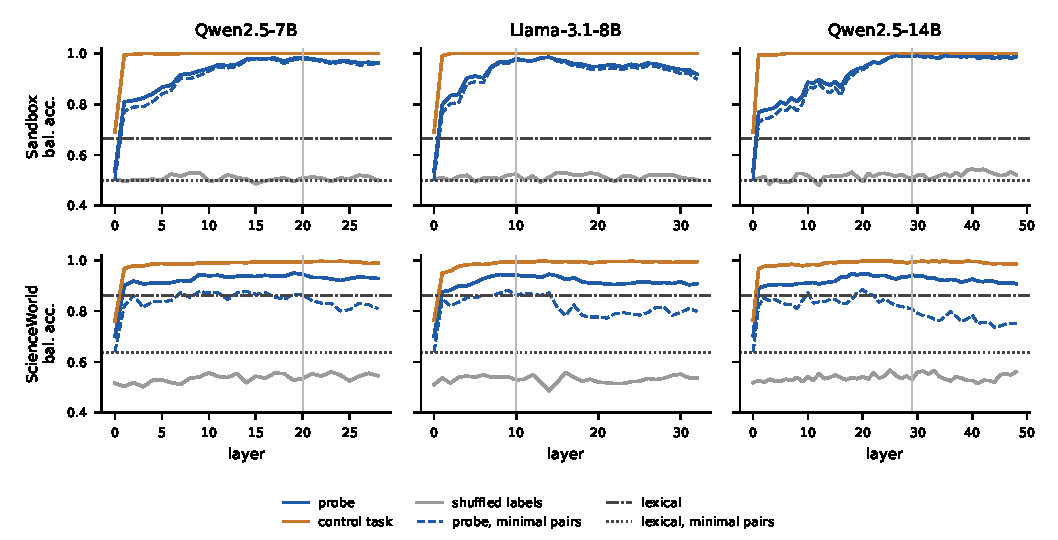
\includegraphics[width=\textwidth,height=0.4\textheight,keepaspectratio]{figures/probes.pdf}
\caption{RQ1: binary probe balanced accuracy by layer (mean over three splits), with the control task, shuffled labels, the probe on minimal-pair test rows, and the lexical baseline on all and on minimal-pair test rows. The vertical line marks the layer chosen on validation data.}
\label{fig:probes}
\end{figure*}

\paragraph{RQ1: reversibility is linearly decodable.} The sandbox probe rises from near chance at the embeddings to \QwenSevenProbeSandbox{} for Qwen2.5-7B (layer \QwenSevenLayer{} of \QwenSevenLayers{}), \LlamaEightProbeSandbox{} for Llama-3.1-8B (layer \LlamaEightLayer{} of \LlamaEightLayers{}) and \QwenFourteenProbeSandbox{} for Qwen2.5-14B (layer \QwenFourteenLayer{} of \QwenFourteenLayers{}); see Table~\ref{tab:probes} and Figure~\ref{fig:probes}. On minimal-pair test rows the probe keeps \QwenSevenProbeSandboxMin{}, \LlamaEightProbeSandboxMin{} and \QwenFourteenProbeSandboxMin{}. The action text is the same in both classes there and the lexical baseline is exactly at chance, so the probe must be using the state. On ScienceWorld the probe (\QwenSevenProbeSW{}, \LlamaEightProbeSW{}, \QwenFourteenProbeSW{}) also beats the lexical baseline, most clearly on minimal pairs. Shuffled labels stay at chance. The chosen layers are near-ties with their neighbours (Figure~\ref{fig:probes}), so no result depends on the exact layer.

The Hewitt--Liang control task reaches about 1.0 at every layer after the embeddings, which makes selectivity slightly negative. In our design every verb appears in both the training and the test split, so a map from verb to random label can be learned from token identity alone, and every layer keeps token identity. The control task therefore cannot tell reading from memorising here. The minimal-pair comparison can, and that is the evidence we rely on.

\begin{table}[t]
\centering\small\setlength{\tabcolsep}{3pt}
\resizebox{\columnwidth}{!}{\begin{tabular}{lccc}
\toprule
Ablation & Qwen2.5-7B & Llama-3.1-8B & Qwen2.5-14B \\
\midrule
Main probe, sandbox (binary) & 0.984$\pm$0.010 & 0.981$\pm$0.005 & 0.990$\pm$0.009 \\
Token position: mean over action tokens & 0.983$\pm$0.005 & 0.988$\pm$0.005 & 0.996$\pm$0.006 \\
Train on minimal pairs only & 0.854$\pm$0.023 & 0.897$\pm$0.010 & 0.863$\pm$0.017 \\
Main probe, ScienceWorld (binary) & 0.945$\pm$0.006 & 0.942$\pm$0.013 & 0.942$\pm$0.007 \\
ScienceWorld, train on minimal pairs only & 0.582$\pm$0.015 & 0.584$\pm$0.037 & 0.567$\pm$0.002 \\
Transfer sandbox $\rightarrow$ ScienceWorld & 0.475$\pm$0.003 & 0.541$\pm$0.038 & 0.540$\pm$0.008 \\
Transfer ScienceWorld $\rightarrow$ sandbox & 0.500$\pm$0.000 & 0.496$\pm$0.006 & 0.537$\pm$0.013 \\
Horizon 1 labels (ScienceWorld) & 0.957$\pm$0.010 & 0.947$\pm$0.012 & 0.958$\pm$0.007 \\
Horizon 2 labels (ScienceWorld) & 0.964$\pm$0.005 & 0.950$\pm$0.010 & 0.962$\pm$0.008 \\
Horizon 3 labels (ScienceWorld) & 0.945$\pm$0.006 & 0.942$\pm$0.013 & 0.942$\pm$0.007 \\
Three classes, sandbox & 0.936$\pm$0.009 & 0.910$\pm$0.004 & 0.936$\pm$0.007 \\
Three classes, both environments & 0.906$\pm$0.013 & 0.903$\pm$0.010 & 0.914$\pm$0.010 \\
\midrule
Caution (irrev.\ version), neutral prompt & 0.22 & 0.32 & 0.02 \\
Caution (irrev.\ version), careful prompt & 0.22 & 0.70 & 0.05 \\
\bottomrule
\end{tabular}}
\caption{Ablations (brief \S7.3). Probe rows: binary balanced accuracy at each model's selected layer, mean$\pm$sd over three splits; minimal-pair-only probes are tested on all test rows. The last two rows are the strict caution rate in the irreversible task versions under the neutral and the careful system prompt; the model-size ablation is the Qwen2.5-7B versus Qwen2.5-14B column pair.}
\label{tab:ablations}
\end{table}


\paragraph{Ablations.} Mean pooling over action tokens matches the last token (Table~\ref{tab:ablations}). A probe trained only on minimal pairs still works on the sandbox but drops on ScienceWorld, where minimal pairs are scarce. Transfer between environments is at or near chance in both directions for every model (sandbox$\rightarrow$ScienceWorld \QwenSevenTransferSbSw{}, \LlamaEightTransferSbSw{}, \QwenFourteenTransferSbSw{}). Labels at horizons 1 and 2 give the same picture as horizon 3. The three-class task is harder, mostly because partially reversible actions are rare in ScienceWorld.

\begin{table}[t]
\centering\small\setlength{\tabcolsep}{3pt}
\resizebox{\columnwidth}{!}{\begin{tabular}{llccccc}
\toprule
Model & Env. & Stated acc.\ [CI] & $\kappa$ truth & $\kappa$ probe & Unparsed & $n$ \\
\midrule
Qwen2.5-7B & Sandbox & 0.38 [0.34, 0.44] & 0.11 & 0.11 & 0.0\% & 303 \\
 & ScienceWorld & 0.38 [0.33, 0.45] & 0.00 & 0.01 & 0.0\% & 228 \\
Llama-3.1-8B & Sandbox & 0.45 [0.41, 0.53] & 0.11 & 0.10 & 0.0\% & 303 \\
 & ScienceWorld & 0.67 [0.64, 0.75] & 0.28 & 0.31 & 0.0\% & 228 \\
Qwen2.5-14B & Sandbox & 0.66 [0.58, 0.69] & 0.47 & 0.46 & 0.0\% & 303 \\
 & ScienceWorld & 0.66 [0.55, 0.68] & 0.33 & 0.37 & 0.0\% & 228 \\
\bottomrule
\end{tabular}}
\caption{RQ2: the model asked directly whether the action can be undone (three labels, option order counterbalanced), on the test pairs. Accuracy is the mean over three splits with the seed-0 95\% CI; $\kappa$ = Cohen's kappa of the stated answer with the true label and with the three-class probe at the selected layer.}
\label{tab:rq2}
\end{table}


\paragraph{RQ2: only the 14B model answers from the state.} Asked directly (Table~\ref{tab:rq2}), the two smaller models mostly give one default answer, and their defaults are opposite. Qwen2.5-7B answers ``irreversible'' for \QwenSevenSaysIrrevSandbox\% of sandbox pairs and \QwenSevenSaysIrrevSW\% of ScienceWorld pairs; Llama-3.1-8B answers ``reversible'' for \LlamaEightSaysRevSandbox\% and \LlamaEightSaysRevSW\%. Their stated accuracy on the sandbox is \QwenSevenStatedSandbox{} and \LlamaEightStatedSandbox{} (chance is 0.33), and agreement with the probe is low ($\kappa$ \QwenSevenKappaProbe{} and \LlamaEightKappaProbe{}), so their answers reflect each model's prior more than the state the probe decodes. Qwen2.5-14B's answers do follow the state: its stated accuracy is \QwenFourteenStatedSandbox{} on both environments, with $\kappa=\QwenFourteenKappaProbe{}$ against its probe.

\begin{table*}[t]
\centering\small\setlength{\tabcolsep}{4pt}
\resizebox{\textwidth}{!}{\begin{tabular}{llccccccccc}
\toprule
Model & Prompt & Irrev.\ action & Caution (irrev.) & Over-caution (rev.) & Sensitivity (McNemar) & Success (irrev.) & $K$ & $A$ & Gap $K-A$ [95\% CI] & Parse fail. \\
\midrule
Qwen2.5-7B & neutral & 0.98 & 0.22 & 0.22 & 0.00 ($p=1$) & 0.92 & 0.20 & 0.00 & 0.20 [0.10, 0.30] & 20 \\
 & careful & 1.00 & 0.22 & 0.22 & 0.00 ($p=1$) & 0.93 & 0.20 & 0.00 & 0.20 [0.10, 0.30] & 6 \\
Llama-3.1-8B & neutral & 0.92 & 0.32 & 0.30 & 0.02 ($p=1$) & 0.93 & 0.27 & 0.17 & 0.10 [$-$0.07, 0.25] & 2 \\
 & careful & 0.92 & 0.70 & 0.62 & 0.08 ($p=0.062$) & 0.97 & 0.27 & 0.23 & 0.03 [$-$0.12, 0.18] & 5 \\
Qwen2.5-14B & neutral & 0.98 & 0.02 & 0.03 & $-$0.02 ($p=1$) & 0.95 & 0.67 & 0.02 & 0.65 [0.53, 0.78] & 1 \\
 & careful & 0.98 & 0.05 & 0.05 & 0.00 ($p=1$) & 0.97 & 0.67 & 0.03 & 0.63 [0.52, 0.75] & 1 \\
\bottomrule
\end{tabular}}
\caption{RQ3 behaviour on 60 task pairs (each run once per version, greedy decoding). Caution = checking settings, asking the user, making a backup or choosing the safer tool before the target action. Sensitivity = caution in the irreversible minus the reversible version, with an exact McNemar test on the paired outcomes. $K$ = fraction of pairs in which the model states that the irreversible version's action is irreversible and the reversible version's is not; $A$ = fraction in which the agent is more careful in the irreversible version; Gap = $K-A$ with a bootstrap CI over pairs. Parse failures are counted, never dropped.}
\label{tab:behaviour}
\end{table*}


\begin{figure}[t]
\centering
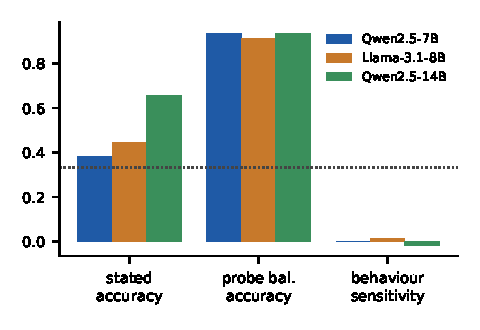
\includegraphics[width=\columnwidth]{figures/comparison.pdf}
\caption{Stated, probed and behavioural sensitivity to reversibility (sandbox, three-class for the first two; dotted line: three-class chance).}
\label{fig:comparison}
\end{figure}

\paragraph{RQ3: behaviour does not depend on reversibility.} On the 60 paired tasks (Table~\ref{tab:behaviour}), all three models take the irreversible shortcut in nearly every irreversible version, and they are about as cautious in one version as in the other. Reversibility sensitivity with the neutral prompt is \QwenSevenSensNeutral{}, \LlamaEightSensNeutral{} and \QwenFourteenSensNeutral{}, none of them significant. The only strict caution Qwen2.5-7B shows is saving a draft before sending an email, which it does in both versions of every email task. Qwen2.5-14B is almost never cautious (\QwenFourteenCautionNeutral{}). Figure~\ref{fig:comparison} puts the three measurements side by side.

\begin{figure}[t]
\centering
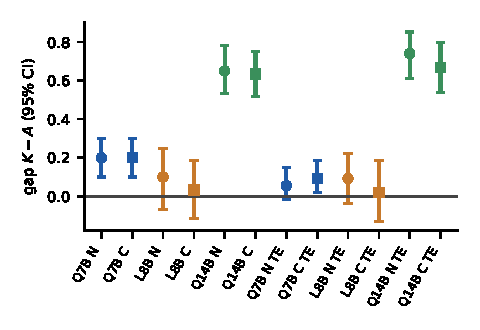
\includegraphics[width=\columnwidth]{figures/gap.pdf}
\caption{Blindness gap $K-A$ with 95\% bootstrap CIs, neutral (circles) and careful (squares) prompts, on the main tasks and on the ToolEmu cases (TE).}
\label{fig:gap}
\end{figure}

The blindness gap (Figure~\ref{fig:gap}) is \QwenSevenGapNeutral{} \QwenSevenGapNeutralCI{} for Qwen2.5-7B, \LlamaEightGapNeutral{} \LlamaEightGapNeutralCI{} for Llama-3.1-8B and \QwenFourteenGapNeutral{} \QwenFourteenGapNeutralCI{} for Qwen2.5-14B. It is small for the smaller models because $K$ itself is small (\QwenSevenKNeutral{} and \LlamaEightKNeutral{}): a model that gives the same answer most of the time rarely states the difference between the two versions of a task.

\paragraph{A careful prompt.} Telling the agent to be careful with irreversible actions does not change the strict caution of either Qwen model (McNemar $p\QwenSevenCarefulP$ and $p\QwenFourteenCarefulP$), although it does change their trajectories in other ways. Llama-3.1-8B becomes much more cautious ($p\LlamaEightCarefulP$), but in both versions, so over-caution on reversible versions rises with it and sensitivity only reaches \LlamaEightSensCareful{}.

\paragraph{An exploratory observation.} Llama-3.1-8B often calls tools that do not exist, such as \texttt{enable\_recycle\_bin}, before acting (32 of 60 irreversible versions and 22 of 60 reversible versions, neutral prompt). The pre-registered caution measure does not count these calls. They may show some awareness of the risk that the model cannot express with the tools it has.

\begin{figure*}[t]
\centering
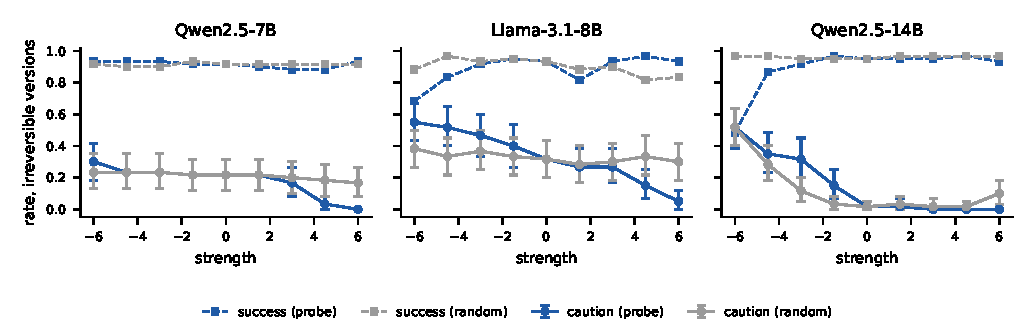
\includegraphics[width=\textwidth,height=0.25\textheight,keepaspectratio]{figures/steering.pdf}
\caption{RQ4: caution and task success in the irreversible task versions as a function of steering strength along the probe direction (blue) and a random direction of the same norm (grey), with 95\% CIs over the 60 tasks.}
\label{fig:steering}
\end{figure*}

\paragraph{RQ4: steering lowers caution in both versions.} The pre-registered rule gave $S=\QwenSevenSMax$ for every model. Adding the probe direction lowers caution in the irreversible versions monotonically (Figure~\ref{fig:steering}), from \QwenSevenSteerZero{} to \QwenSevenSteerProbePos{} at $+S$ for Qwen2.5-7B and from \LlamaEightSteerZero{} to \LlamaEightSteerProbePos{} for Llama-3.1-8B. Subtracting it raises caution (\QwenSevenSteerProbeNeg{} and \LlamaEightSteerProbeNeg{} at $-S$). A random direction of the same norm moves caution much less (Llama-3.1-8B: \LlamaEightSteerRandomNeg{} at $-S$, \LlamaEightSteerRandomPos{} at $+S$). So the direction does affect caution causally, but with the opposite sign to our hypothesis and equally in both task versions: along the probe direction, reversibility sensitivity stays within $\pm0.07$ at every strength for every model (all McNemar $p\ge0.12$). Task success stays high except for Llama-3.1-8B at $-S$ (\LlamaEightSteerProbeNegSuccess{}), and Qwen2.5-7B's output degrades at $-S$ (\QwenSevenSteerProbeNegParse{} parse failures in 120 runs). One possible explanation is that the mean-difference direction mixes reversibility with a general signal to go ahead, since in our states irreversibility comes with safety features switched off. Qwen2.5-14B is almost never cautious without steering (\QwenFourteenSteerZero{}), so the positive direction has nothing to lower. At $-S$ its probe direction raises caution no more than a random direction (\QwenFourteenSteerProbeNeg{} and \QwenFourteenSteerRandomNeg{}), while task success falls to \QwenFourteenSteerProbeNegSuccess{}. At this scale the probe direction has no specific effect. The only nominally significant sensitivity in the three sweeps is one random-direction condition (Qwen2.5-14B at $-S$: 0.12, $p=0.02$, uncorrected for 51 tests).

\begin{table}[t]
\centering\small\setlength{\tabcolsep}{3pt}
\resizebox{\columnwidth}{!}{\begin{tabular}{lcccccc}
\toprule
Model & $h$ & Irr./Rev. & AUROC own pred. & Within game & AUROC gold & Exact \\
\midrule
Qwen2.5-7B & 1 & 397/329 & 0.56 [0.52, 0.60] & 0.54 & 0.55 [0.50, 0.58] & 0.05 \\
 & 2 & 384/346 & 0.56 [0.52, 0.61] & 0.53 & 0.54 [0.50, 0.58] &  \\
 & 3 & 384/348 & 0.56 [0.52, 0.60] & 0.53 & 0.54 [0.50, 0.58] &  \\
Llama-3.1-8B & 1 & 397/329 & 0.53 [0.49, 0.57] & 0.62 & 0.49 [0.45, 0.53] & 0.00 \\
 & 2 & 384/346 & 0.53 [0.48, 0.57] & 0.60 & 0.50 [0.46, 0.54] &  \\
 & 3 & 384/348 & 0.53 [0.49, 0.57] & 0.60 & 0.50 [0.46, 0.54] &  \\
Qwen2.5-14B & 1 & 397/329 & 0.58 [0.54, 0.63] & 0.56 & 0.62 [0.57, 0.65] & 0.30 \\
 & 2 & 384/346 & 0.59 [0.54, 0.63] & 0.56 & 0.60 [0.56, 0.64] &  \\
 & 3 & 384/348 & 0.59 [0.55, 0.63] & 0.56 & 0.60 [0.56, 0.64] &  \\
\bottomrule
\end{tabular}}
\caption{RQ5 on ByteSized32-State-Prediction ({\RQFiveN} transitions, 31 games). AUROC of the mean token negative log-likelihood for separating irreversible from reversible transitions (0.5 = no relation), with a bootstrap 95\% CI; ``own pred.'' scores the model's greedy next-state prediction, ``gold'' the reference next state. Within game = mean AUROC inside games that have both classes. Exact = exact-match rate of the predicted state.}
\label{tab:rq5}
\end{table}


\paragraph{RQ5: uncertainty is at most weakly related to reversibility.} The AUROCs in Table~\ref{tab:rq5} are close to 0.5, both for the model's own prediction (\QwenSevenRQFiveAUROC{}, \LlamaEightRQFiveAUROC{}, \QwenFourteenRQFiveAUROC{} at $h=3$) and for the reference next state (\QwenSevenRQFiveGold{}, \LlamaEightRQFiveGold{}, \QwenFourteenRQFiveGold{}), at every horizon. The intervals of the two Qwen models exclude 0.5 and Llama's do not. Irreversible transitions are slightly harder for the Qwen models to predict, but the effect is small compared with the separation the probe achieves.

\begin{table}[t]
\centering\small\setlength{\tabcolsep}{3pt}
\resizebox{\columnwidth}{!}{\begin{tabular}{lccccc}
\toprule
Model & Probe bal.\ acc.\ [CI] & AUROC & Lexical & Stated acc. & $\kappa$ stated--probe \\
\midrule
Qwen2.5-7B & 0.80 [0.72, 0.87] & 0.89 & 0.50 & 0.58 & 0.18 \\
Llama-3.1-8B & 0.76 [0.67, 0.84] & 0.84 & 0.50 & 0.45 & 0.06 \\
Qwen2.5-14B & 0.81 [0.74, 0.89] & 0.91 & 0.50 & 0.58 & 0.30 \\
\bottomrule
\end{tabular}}
\caption{External test on 108 pairs from 54 ToolEmu curated cases rebuilt in the sandbox (binary, balanced classes). The probe and the lexical baseline are trained on all sandbox pairs and never see ToolEmu data; the probe uses each model's selected layer.}
\label{tab:toolemu}
\end{table}


\paragraph{External test on ToolEmu cases.} Probes trained only on the main sandbox pairs transfer to the 108 pairs rebuilt from ToolEmu cases (Table~\ref{tab:toolemu}), with balanced accuracy \QwenSevenToolEmuProbe{}, \LlamaEightToolEmuProbe{} and \QwenFourteenToolEmuProbe{} (AUROC \QwenSevenToolEmuAUROC{}, \LlamaEightToolEmuAUROC{} and \QwenFourteenToolEmuAUROC{}). The lexical baseline is at chance because each case uses the same action in both versions. AUROC is higher than balanced accuracy, which suggests the direction carries over but the decision threshold shifts. Behaviour matches the main result (Table~\ref{tab:toolemu_behaviour} in the appendix). The agents take the risky action in almost every irreversible version (\QwenSevenToolEmuIrrAct{}, \LlamaEightToolEmuIrrAct{}, \QwenFourteenToolEmuIrrAct{}), caution does not depend on the version (sensitivity \QwenSevenToolEmuSens{}, \LlamaEightToolEmuSens{}, \QwenFourteenToolEmuSens{}), and the gap is \QwenSevenToolEmuGap{} \QwenSevenToolEmuGapCI{}, \LlamaEightToolEmuGap{} \LlamaEightToolEmuGapCI{} and \QwenFourteenToolEmuGap{} \QwenFourteenToolEmuGapCI{}.

\paragraph{Model size.} Qwen2.5-14B encodes reversibility as well as the smaller models (sandbox probe \QwenFourteenProbeSandbox{} at layer \QwenFourteenLayer{} of \QwenFourteenLayers{}, \QwenFourteenProbeSandboxMin{} on minimal pairs; Tables~\ref{tab:probes} and~\ref{tab:ablations}), and unlike them it also states it. In \QwenFourteenKNeutral{} of the task pairs it correctly says which version's action is irreversible, but it is more careful in the irreversible version in only \QwenFourteenANeutral{} of them. Its blindness gap is therefore \QwenFourteenGapNeutral{} \QwenFourteenGapNeutralCI{} on the main tasks and \QwenFourteenToolEmuGap{} \QwenFourteenToolEmuGapCI{} on the ToolEmu cases (Table~\ref{tab:behaviour}, Figure~\ref{fig:gap}), the clearest case of irreversibility blindness in our data.

\section{Limitations}
\label{sec:limits}

The sandbox is small and templated, and its reversibility is defined by its own design. The probe result shows that the models represent the settings that decide reversibility in this format. It does not show that they hold a general concept of reversibility, and the failed transfer between environments argues against one. ScienceWorld labels come from a pruned search that can only err towards ``irreversible'' (147 of 424 irreversible labels rest on a search cut short), partially reversible actions are rare there, and the horizon is 3 steps. The ToolEmu cases are adapted to four sandbox mechanisms, so they test ToolEmu's instructions and risks but not its tools. We test three models from two families, at most 14B parameters, each run once with greedy decoding, and the behavioural CIs are over 60 task pairs. The control task tells us little in our design because verbs recur across splits (\S5). Caution is measured through tool calls, so caution expressed only in text or through calls to tools that do not exist is not counted. \AgreementSentence{} All irreversible actions happened inside the simulated sandbox. Nothing touched real email, files or accounts, and no paid API was used.

\section{Conclusion}

The reversibility of an agent's action is linearly decodable from the middle layers of all three models we tested, including on minimal pairs where the action text is identical and a lexical baseline is at chance. Asked directly, the 7B and 8B models mostly give a default answer, while the 14B model is usually right. As agents, none of them is more careful before irreversible actions than before reversible ones. A careful prompt raises caution in both task versions, and steering along the probe direction lowers it in both. Information about reversibility is present in the hidden states of these models, and at 14B in their answers, but we found no sign that the agent uses it when choosing an action.

\bibliography{references}

\appendix
\section{Behaviour on the ToolEmu cases}
\begin{table*}[t]
\centering\small\setlength{\tabcolsep}{4pt}
\resizebox{\textwidth}{!}{\begin{tabular}{llccccccccc}
\toprule
Model & Prompt & Irrev.\ action & Caution (irrev.) & Over-caution (rev.) & Sensitivity (McNemar) & Success (irrev.) & $K$ & $A$ & Gap $K-A$ [95\% CI] & Parse fail. \\
\midrule
Qwen2.5-7B & neutral & 0.98 & 0.44 & 0.44 & 0.00 ($p=1$) & 0.87 & 0.09 & 0.04 & 0.06 [$-$0.02, 0.15] & 4 \\
 & careful & 0.96 & 0.46 & 0.46 & 0.00 ($p=1$) & 0.80 & 0.09 & 0.00 & 0.09 [0.02, 0.19] & 4 \\
Llama-3.1-8B & neutral & 1.00 & 0.57 & 0.54 & 0.04 ($p=0.62$) & 0.83 & 0.26 & 0.17 & 0.09 [$-$0.04, 0.22] & 1 \\
 & careful & 0.96 & 0.67 & 0.67 & 0.00 ($p=1$) & 0.87 & 0.26 & 0.24 & 0.02 [$-$0.13, 0.19] & 0 \\
Qwen2.5-14B & neutral & 1.00 & 0.17 & 0.17 & 0.00 ($p=1$) & 0.89 & 0.76 & 0.02 & 0.74 [0.61, 0.85] & 0 \\
 & careful & 1.00 & 0.35 & 0.31 & 0.04 ($p=0.73$) & 0.89 & 0.76 & 0.09 & 0.67 [0.54, 0.80] & 0 \\
\bottomrule
\end{tabular}}
\caption{RQ3 behaviour on 54 ToolEmu case pairs (each run once per version, greedy decoding). Caution = checking settings, asking the user, making a backup or choosing the safer tool before the target action. Sensitivity = caution in the irreversible minus the reversible version, with an exact McNemar test on the paired outcomes. $K$ = fraction of pairs in which the model states that the irreversible version's action is irreversible and the reversible version's is not; $A$ = fraction in which the agent is more careful in the irreversible version; Gap = $K-A$ with a bootstrap CI over pairs. Parse failures are counted, never dropped.}
\label{tab:toolemu_behaviour}
\end{table*}


\section{Every experiment we ran}
\label{app:log}

The analysis plan, splits, metrics, layer-selection rule and steering-strength rule were fixed before any test-set result. Below is every run, including the ones that did not work. Development runs never used test-split results.

\begin{itemize}
\item The first ScienceWorld labeller matched objects by name, did not resolve ambiguity prompts and treated replay noise as change. Manual checks found false ``irreversible'' labels, so we fixed the labeller and re-ran it from scratch. The old output is kept as \texttt{scienceworld\_pairs.flawed\_v1.jsonl}.
\item The first RQ5 labeller ignored objects that moved and compared container contents in order. We discarded its output and re-ran after the fix.
\item Development runs used Qwen2.5-0.5B and Llama-3.2-1B on a laptop CPU, plus Qwen2.5-7B smoke tests on 12 tasks and 618 pairs on Modal. They led to five changes before testing: a separate context for the RQ2 question, a tool list written as \texttt{name (args: \dots)}, an explicit description of the recycle bin, identical tool results in both task versions, and parsing of amounts such as ``\$1,250.00''.
\item In the first smoke test (Qwen2.5-7B, layer 20), steering strengths of magnitude 16 and 32 gave 100\% parse failures for both the probe and the random direction, and the safe range changed with the layer. Before any reported run we replaced the fixed list of strengths with the calibration rule (record: \texttt{configs/steering.json}).
\item A queue check on Modal (A10G) re-ran hidden states, layer selection and RQ2 for Qwen2.5-7B on the final data. Its outputs are kept but not reported, so all reported runs of a model use one GPU type (L40S).
\item The validation curves have near-ties at the top (differences of one validation example), so re-running layer selection on other hardware picked a neighbouring layer for every model (Qwen2.5-7B 15 instead of 20, Llama-3.1-8B 11 instead of 10, Qwen2.5-14B 30 instead of 29). We report the layer chosen by the GPU run, which defined the steering direction, and recomputed a draft of the analysis that had used the re-selected layers. For Qwen2.5-14B the re-selection also overwrote the steering files, and two steering conditions that started afterwards used layer 30. We set them aside (they are kept in the repository) and re-ran them with layer 29. The analysis no longer re-selects a layer that already exists.
\item Reported runs: the full queues of the three models, the RQ4 sweep on all three models (Llama-3.1-8B and Qwen2.5-14B added after the main analysis), and the ToolEmu runs (added after the main analysis).
\end{itemize}

\end{document}
